\newpage
\clearpage

\section{Redes Neurais Convolucionais}
\label{cnn}

Dentre os diversos tipos de redes de aprendizado profundo, as mais amplamente utilizadas atualmente para lidar com visão computacional, processamento de imagens e possuindo um valor notável para o trabalho com dados espaciais \citep{Goodfellow2016, ponti2018funciona, Ghosh2019}, destacam-se as \textit{Convolutional Neural Networks} (CNNs) \citep{LeCun1999}. As CNNs recebem esse nome por empregarem camadas convolucionais, sendo especialmente proeminentes e eficazes nesses contextos.

É inegável que as CNNs são consideradas o estado-da-arte em várias competições \citep{Parkhi2015}, além de serem modelos bioinspirados de sucesso \citep{Goodfellow2016}. Elas são capazes de simular pontos cerebrais responsáveis pela interpretação de impulsos visuais, reproduzindo propriedades do córtex visual. Além disso, essas redes têm a capacidade de extrair diferentes características, utilizando operações de \textit{pooling}, que serão detalhadas na Seção \ref{cnn:pooling}.

Entre a vasta gama de arquiteturas disponíveis para as CNNs, destacam-se algumas das mais influentes: AlexNet \citep{krizhevsky2012imagenet}, VGGNet \citep{Simonyan2015}, ResNet \citep{He2016}, GoogLeNet \citep{Szegedy2015}, MobileNet \citep{Howard2017} e DenseNet \citep{Huang2017}. Essas arquiteturas possuem contribuições significativas e têm sido aplicadas em uma variedade de contextos, cada uma com suas características e aplicações específicas.

Um modelo indicando uma entrada, as camadas convolucionais iniciais e finais, que são utilizadas para extração de atributos, bem como o sistema de \textit{pooling} e a camada de saída (ou camada densa) são representados por meio da Figura \ref{cnn:fig:10}:

\begin{figure}[H]
    \centering
    \caption{Modelo de CNN.}
    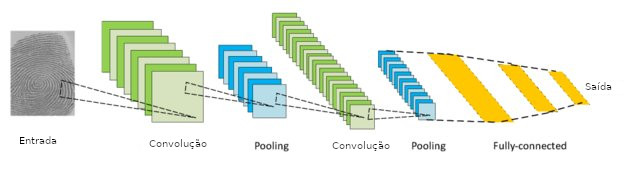
\includegraphics[width=1\linewidth]{recursos/imagens/deep/cnn.jpg}
    \label{cnn:fig:10}

    Fonte: retirada e adaptado de \cite{Minaee2021DeepClassification}.
\end{figure}

Dessa forma, nas seções seguintes, os elementos fundamentais que compõem uma rede neural convolucional serão minuciosamente explorados. Estes incluem a camada convolucional (Seção \ref{cnn:conv}), a camada de \textit{pooling} (Seção \ref{cnn:pooling}), o componente \textit{dropout} (Seção \ref{cnn:dropout}) e a camada de saída (Seção \ref{cnn:output}) da rede. Adicionalmente, serão abordados temas complementares que impactam significativamente no desempenho das CNNs, tais como transferência de aprendizado (Seção \ref{cnn:transfer}) e aumento de dados (Seção \ref{cnn:augment}). Por fim, será explorada uma das arquiteturas que exerceu considerável influência na evolução desse campo, a VGG (Seção \ref{cnn:vgg}).


\subsection{Camada Convolucional}
\label{cnn:conv}

Na arquitetura das CNNs, a modelagem de cada neurônio presente na camada convolucional envolve a aplicação de um filtro na imagem em análise \citep{ponti2018funciona}. Esses filtros são compostos por pesos e a operação de convolução é categorizada como uma operação linear \citep{Goodfellow2016}, resultando nos chamados mapas de características (\textit{feature maps} em inglês).

É fundamental destacar que entre as camadas convolucionais existem $N$ filtros, cujos parâmetros são definidos de acordo com a natureza do problema em questão, utilizando seus resultados para formar tensores, conforme comentado por \cite{ponti2018funciona}.

A operação de convolução pode ser ilustrada pela Figura \ref{cnn:fig:6}, onde uma imagem de entrada é representada pela matriz de maior escala. Nesse processo, utiliza-se uma janela, conhecida como \textit{kernel}, composta por pesos, que convolui com a matriz de entrada para extrair características específicas da imagem, mantendo a integridade das informações sobre sua disposição espacial.

Essas operações são fundamentais nas CNNs, pois permitem a extração eficiente de características importantes das imagens, o que é crucial para a eficácia e a precisão do processo de aprendizado da rede neural convolucional.

\begin{figure}[H]
    \centering
    \caption{Representação do processo de convolução.}
    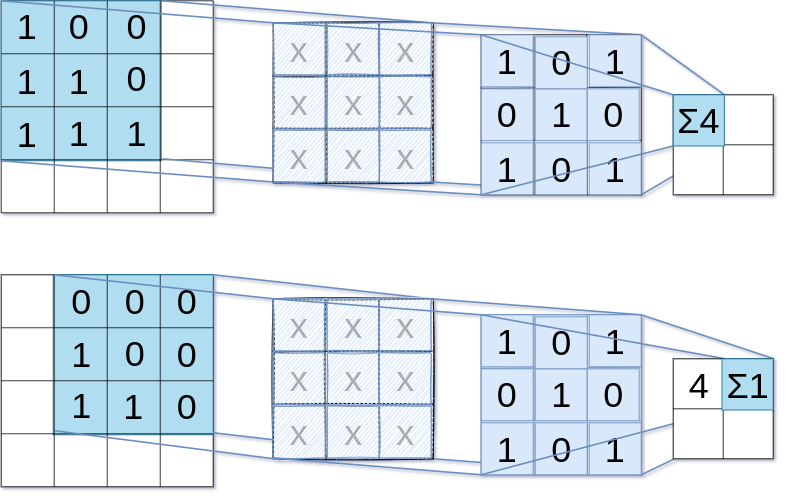
\includegraphics[width=1\linewidth]{recursos/imagens/deep/2d_convolution.png}
    \label{cnn:fig:6}

    Fonte: do próprio autor.
\end{figure}

Ainda na Figura \ref{cnn:fig:6}, é possível observar o processo de deslizamento do \textit{kernel} durante a operação de convolução, resultando em um dos valores presentes na saída. Esse processo é repetido até que toda a imagem seja percorrida, de maneira sequencial da esquerda para a direita e de cima para baixo, movimentando-se através das linhas e colunas.

É crucial ressaltar que a convolução é um processo de média móvel, isto é, implica no cálculo da média ponderada de uma janela específica na imagem, correspondente ao tamanho do \textit{kernel} utilizado. Nesse contexto, o \textit{kernel} define os pesos aplicados aos pontos da janela. Consequentemente, à medida que o \textit{kernel} desliza pela imagem, novas janelas são definidas e suas médias ponderadas são computadas.

Essa abordagem de convolução, com seu deslizamento e cálculo ponderado, é essencial para a extração de informações significativas da imagem, contribuindo para a identificação de padrões relevantes ao longo do processo de aprendizado da rede neural convolucional.


\subsection{Camada de \textit{Pooling}}
\label{cnn:pooling}

Dentro do contexto das camadas de \textit{pooling}, é relevante mencionar que essas camadas são amplamente empregadas nas CNNs com o propósito de reduzir o tempo de treinamento, já que sua função primária é diminuir a dimensionalidade dos mapas de características entre as iterações da rede.

É digno de nota que a adaptação e evolução desses métodos de \textit{pooling} têm recebido crescente atenção na literatura recente \citep{Sabri2020AClassificationb, Zafar2022ANetworks}. Cada modificação busca contribuir para a solução de problemas específicos, evidenciando o constante desenvolvimento dessas técnicas na área de visão computacional e aprendizado profundo.

Ademais, vale ressaltar que na literatura existem diversos modelos de \textit{pooling} que se destacam no uso em redes de aprendizado profundo. Entre eles, destacam-se o \textit{max pooling}, \textit{average pooling}, \textit{median pooling} e \textit{weighted average} \citep{Goodfellow2016}. Há também outros modelos comumente encontrados em redes mais modernas, como o \textit{global average pooling}, \textit{global max pooling} e \textit{astrous spatial pyramid pooling}, principalmente em aplicações de segmentação ou com propostas alternativas. Alguns desses modelos serão discutidos a seguir.

\subsubsection{\textit{Max Pooling}}
\label{cnn:pooling:max_pooling}
O \textit{max pooling} é uma das técnicas mais conhecidas e amplamente utilizadas para realizar o \textit{pooling} em CNNs \citep{Zafar2022ANetworks, Paul2019DimensionalityPooling}. Esta técnica é preferida devido à sua simplicidade, não exigindo ajuste de parâmetros, além de atender de forma eficiente à necessidade de reduzir a dimensionalidade das entradas \citep{Boureau2010ARecognition}.

O funcionamento do \textit{max pooling}, denotado por $f_{\max}(\boldsymbol{X})$, pode ser representado pela Equação \ref{cnn:eq:pooling:max_pooling}:

\begin{equation}
\label{cnn:eq:pooling:max_pooling}
f_{\max}(\boldsymbol{X})_{i, j, k} = \max_{m, n} X_{i \cdot s_x + m, j \cdot s_{y} + n, k}.
\end{equation}

Nesta equação, $\boldsymbol{X}$ representa o valor de entrada, $(i, j)$ são os índices do valor de saída e $k$ é a quantidade de canais (ou camadas) associadas ao valor de entrada. Além disso, $s_{x}$ e $s_{y}$ representam os tamanhos de deslocamento (ou \textit{stride}) horizontal e vertical, respectivamente. O resultado da operação de \textit{max pooling} é obtido utilizando um \textit{kernel} como ilustrado na Figura \ref{cnn:fig:7}, onde a técnica captura apenas os maiores valores do mapa de características.

\begin{figure}[H]
    \centering
    \caption{\textit{Max pooling}.}
    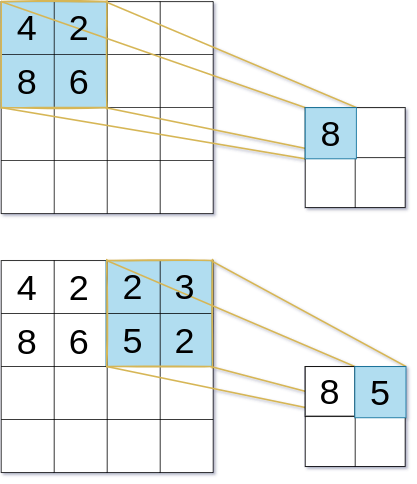
\includegraphics[width=0.5\linewidth]{recursos/imagens/deep/max_pooling.png}
    \label{cnn:fig:7}

    Fonte: do próprio autor.
\end{figure}

É relevante destacar que a aplicação da técnica de \textit{max pooling} adiciona uma leve invariância por translação ao processo. No entanto, de modo geral, isso não afeta de maneira significativa os valores de saída da camada de \textit{pooling} \citep{Boureau2010ARecognition}.

A técnica de \textit{max pooling} é conhecida por preservar características importantes da entrada, ao mesmo tempo em que reduz a dimensionalidade dos mapas de características, tornando-os mais computacionalmente eficientes e facilitando a detecção de padrões por camadas subsequentes da rede neural convolucional. Todavia, essa técnica não se demonstra adequada quando se trata da preservação de espacialidade da entradas \citep{Liu2019Multi-LevelNetworks}.

\subsubsection{\textit{Average Pooling}}
\label{cnn:pooling:avg_pooling}
A técnica de \textit{average pooling}, semelhante à técnica de \textit{max pooling} descrita na Seção \ref{cnn:pooling:max_pooling}, é considerada uma técnica estabelecida e tradicional para aplicação em CNNs \citep{Zafar2022ANetworks, Paul2019DimensionalityPooling}. O funcionamento de ambas as técnicas é bastante semelhante, diferenciando-se principalmente pela aplicação da média em vez da função $\max$ para obter o resultado do \textit{Average Pooling}, denotado por $f_{avg}(\boldsymbol{X})$, conforme ilustrado na Equação \ref{cnn:eq:pooling:avg_pooling}:

\begin{equation}
    \label{cnn:eq:pooling:avg_pooling}
    f_{avg}(\boldsymbol{X})_{i, j, k} = \frac{1}{f{x} \cdot f_{y}} \sum_{m, n} X_{i \cdot s_x + m, j \cdot s_{y} + n, k}.
\end{equation}

Nesta equação, $\boldsymbol{X}$ representa o valor de entrada, $(i, j)$ são os índices do valor de saída e $k$ é o número de camadas. Os parâmetros $s_x$ e $s_y$ representam os valores de \textit{stride} vertical e horizontal, respectivamente, enquanto os tamanhos dos filtros $f_x$ e $f_y$ determinam a janela de \textit{pooling}, centrada nos índices de saída $(i,j)$. Uma representação visual dessa fórmula é ilustrada na Figura \ref{cnn:fig:avg_pooling}.

\begin{figure}[H]
    \centering
    \caption{\textit{Average pooling}.}
    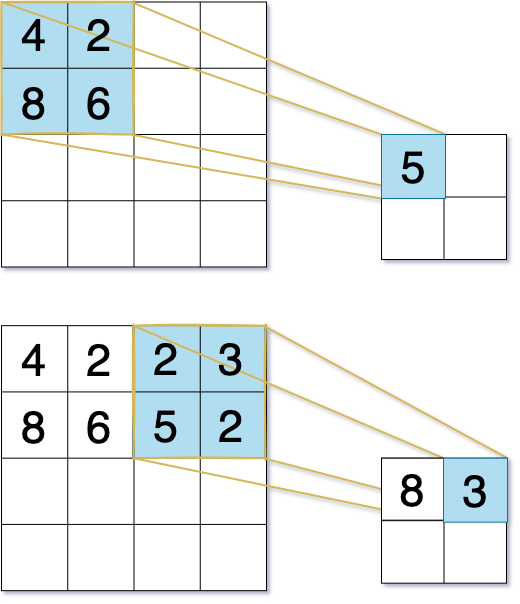
\includegraphics[width=0.5\linewidth]{recursos/imagens/deep/avgpooling.png}
    \label{cnn:fig:avg_pooling}

    Fonte: do próprio autor.
\end{figure}

Por fim, é relevante mencionar que o resultado visual obtido pelo \textit{average pooling} tende a extrair características de maneira mais suave do que o \textit{max pooling}. Enquanto o \textit{max pooling} enfatiza características mais proeminentes, como bordas, o método de \textit{average pooling} tende a extrair características mais suaves, como informações relacionadas às cores. Essa técnica foi utilizada na primeira rede neural profunda baseada em convolução \citep{LeCun1998Gradient-basedRecognition}. Contudo, observam-se desafios semelhantes em relação à preservação da espacialidade das entradas \citep{Liu2019Multi-LevelNetworks}, como ocorre também no algoritmo de \textit{max pooling}.

\subsubsection{\textit{Global Average Pooling}}
\label{cnn:pooling:global_avg_pooling}
A técnica de \textit{Global Average Pooling}, por sua vez, permite a redução dos mapas de características a um único valor por camada, como ilustrado na Figura \ref{cnn:fig:8}.

\begin{figure}[H]
    \centering
    \caption{\textit{Global Average Pooling}.}
    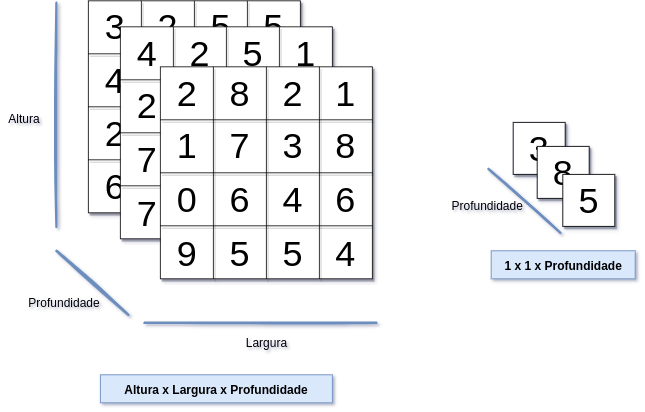
\includegraphics[height=3in]{recursos/imagens/deep/global_average_pooling.png}
    \label{cnn:fig:8}
    
    \caption*{Fonte: do próprio autor.}
\end{figure}

Neste caso, percebe-se que essa técnica é uma variação do \textit{Average Pooling}. Em vez de usar um \textit{kernel} e \textit{strides}, o \textit{Global Average Pooling} aplica a média em todos os valores de entrada. Isso pode ser descrito pela Equação \ref{cnn:eq:pooling:gavg_pooling}:

\begin{equation}
    \label{cnn:eq:pooling:gavg_pooling}
    f_{\text{global avg}}(\boldsymbol{X})_{k} = f_{avg}(\boldsymbol{X}:,:,k),
\end{equation}
onde $k$ representa o índice das camadas e $\boldsymbol{X}$ denota o valor de entrada.

É importante ressaltar que o \textit{Global Average Pooling} também pode ser empregado como uma operação para substituir as camadas totalmente conectadas (em inglês, \textit{fully connected layers}) em CNNs. Nessa abordagem, o método utiliza a média de cada mapa de características para alimentar uma camada de saída com Softmax, que será discutida na Seção \ref{cnn:output}, como foi realizado no trabalho de \cite{Kumar2021Multi-classPooling}.

\subsubsection{\textit{Global Max Pooling}}
\label{cnn:pooling:global_max_pooling}

O método de \textit{Global Max Pooling} possui semelhanças em comparação com os métodos de \textit{Max Pooling} e \textit{Global Average Pooling}. Este método aplica a função de maximização ao longo de todo o mapa de características de cada camada dos valores de entrada, como pode ser visualizado na Equação \ref{cnn:eq:pooling:gmax_pooling}.

\begin{equation}
    \label{cnn:eq:pooling:gmax_pooling}
    f_{\text{global max}}(\boldsymbol{X})_{k} = f_{max}(\boldsymbol{X}:,:,k),
\end{equation}
onde $k$ representa o índice das camadas e $\boldsymbol{X}$ denota o valor de entrada. Essa representação também pode ser exemplificada por meio da Figura \ref{cnn:fig:gmax_pooling}.

\begin{figure}[H]
    \centering
    \caption{\textit{Global Max Pooling}.}
    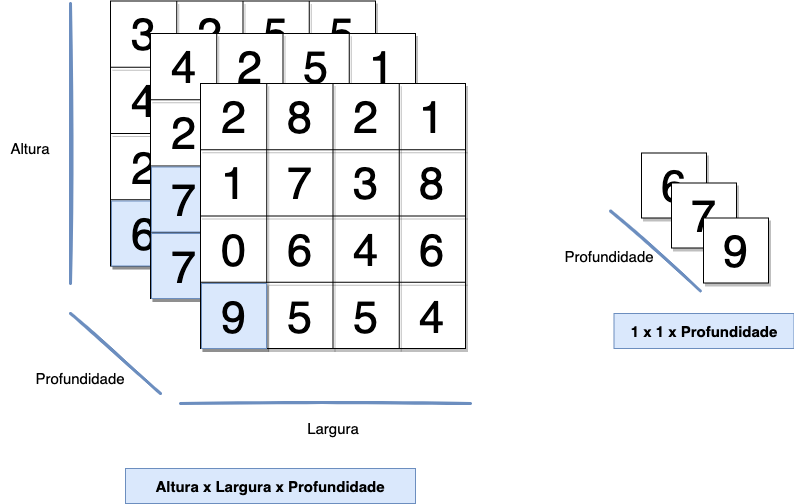
\includegraphics[height=3in]{recursos/imagens/deep/global_max_pooling.png}
    \label{cnn:fig:gmax_pooling}
    
    \caption*{Fonte: do próprio autor.}
\end{figure}

Entretanto, é crucial ressaltar que os métodos convencionais não preservam informações espaciais. Isso se aplica ainda mais aos métodos globais, os quais resumem toda a representação da entrada em um único valor \citep{Christlein2019DeepPooling}. Essa perda de informações espaciais pode ser limitante em algumas tarefas, especialmente em contextos onde a disposição e a relação entre os elementos na entrada têm um papel significativo na análise ou no reconhecimento de padrões.

\subsubsection{\textit{Atrous Spatial Pyramid Pooling}(ASPP)}
\label{cnn:pooling:aspp}
Além da proposta de preservação de escala, embora ainda sem manter a espacialidade, foi introduzido o método \textit{Atrous Spatial Pyramid Pooling} (ASPP) por \cite{Chen2018}. Este tipo de operação de \textit{pooling} está intrinsecamente ligado às segmentações semânticas \citep{Mohan2020} (que serão discutidas na Seção \ref{semantic}). A principal vantagem desse algoritmo é a capacidade de capturar objetos e contexto relevantes da imagem em várias escalas distintas. Essa funcionalidade está associada à re-amostragem utilizando convoluções com diferentes taxas de dilatação para cada \textit{kernel}, permitindo explorar um mapa de características com múltiplos campos de visão antes mesmo do processo de convolução \citep{Chen2018}. Um exemplo desse módulo pode ser visualizado na Figura \ref{cnn:fig:aspp}.

\begin{figure}[H]
    \centering
    \caption{Exemplo ilustrativo do ASPP.}
    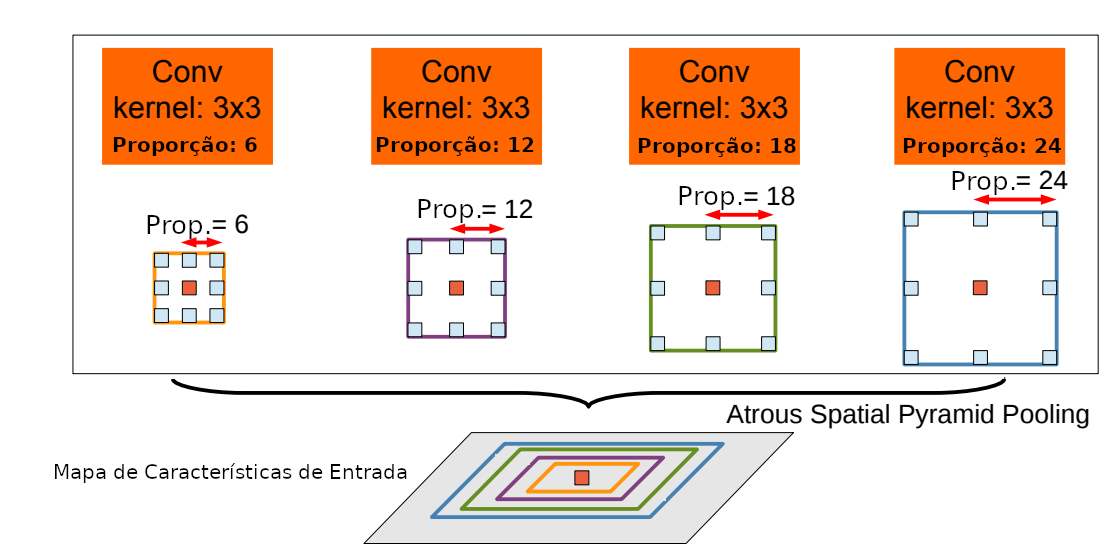
\includegraphics[width=1\textwidth]{recursos/imagens/proposal/aspp.png}
    \label{cnn:fig:aspp}

    Fonte: Adaptado de \cite{Chen2018}.
\end{figure}

O funcionamento do ASPP, que realiza ajustes no mapa de características para calcular informações em múltiplas escalas, pode ser expresso pela Equação \ref{cnn:eq:pooling:aspp}, proposta por \cite{Chen2018}:

\begin{equation}
    \label{cnn:eq:pooling:aspp}
    y[i] = \sum_{k}x[i + r \cdot k]w [k],
\end{equation}
onde $r$ representa uma taxa de dilatação que determina as \textit{strides} para amostrar o mapa de características de entrada $x$, tendo que para cada pixel $i$ na saída $y$ e com o filtro $w$, a convolução dilatada (em inglês, \textit{atrous convolution}) sendo aplicada.

\subsection{\textit{Dropout}}
\label{cnn:dropout}

Dentre as estratégias para mitigar o \textit{overfitting} ,citado na Seção \ref{deep:overunder}, destaca-se a técnica de \textit{dropout} \citep{Goodfellow2016}. Esta técnica, embora não seja aplicada durante a fase de testes, consiste no desligamento aleatório de neurônios em camadas ocultas de uma rede CNN. O propósito do \textit{dropout} é reduzir o viés dos neurônios e aumentar a importância dos neurônios restantes.

O processo de \textit{dropout} é ilustrado na Figura \ref{cnn:fig:9}, mostrando apenas as conexões entre os neurônios restantes, no lado direito da Figura \ref{cnn:fig:9}.

\begin{figure}[H]
    \centering
    \caption{Processo de \textit{dropout}.}
    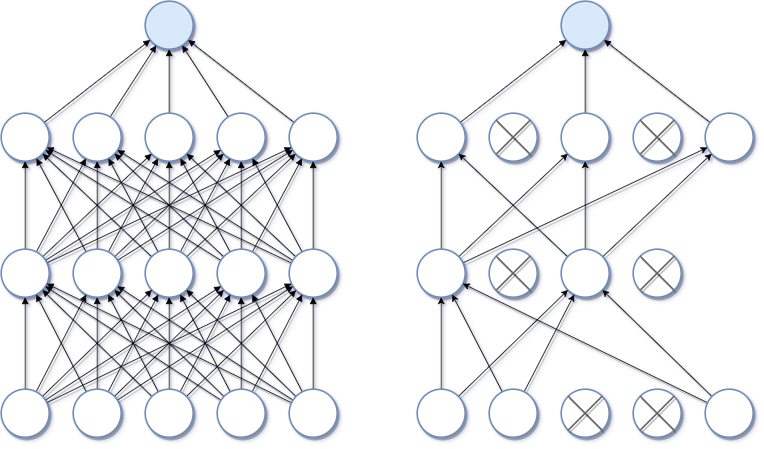
\includegraphics[width=1\linewidth]{recursos/imagens/deep/dropout.png}
    \label{cnn:fig:9}

     Fonte: do próprio autor.
\end{figure}

A técnica de \textit{dropout} é uma estratégia eficaz para regularização em redes neurais, pois ajuda a evitar que a rede se ajuste excessivamente aos dados de treinamento, tornando-a mais capaz de generalizar para dados novos e não vistos durante o treinamento.

\subsection{Camada de Saída}
\label{cnn:output}

Após a composição de várias camadas de convolução, utilizando filtros, e a aplicação de camadas de \textit{pooling}, os modelos de CNN geralmente incluem uma camada de saída, também conhecida como camada densa. Esta camada é fundamental para a determinação das classes identificadas na imagem. Vale destacar que essa camada não tem um impacto significativo no desempenho em relação ao tempo de convergência do modelo, nem interfere no progresso e evolução do processo de treinamento, sendo que o processo de inferência é muito similar ao usado pelas CNNs na Seção \ref{cnn}.

Por fim, para gerar a saída final, é comum utilizar funções de ativação como a Softmax (abordada na Seção \ref{deep:soft}). A aplicação da Softmax permite a identificação da classe de um objeto específico em uma imagem, por exemplo. Essa função de ativação é utilizada para a tarefa de classificação, fornecendo as probabilidades de pertencimento a cada classe no conjunto de dados.


\subsection{Transferência de Aprendizado}
\label{cnn:transfer}

\subsection{Aumento de Dados}
\label{cnn:augment}

\subsection{VGG-16}
\label{cnn:vgg}
\citep{Simonyan2015}

\subsection{Considerações Finais do Capítulo}
\label{cnn:conclusion}
